\documentclass[11pt,oneside]{article}

\usepackage{amsmath,amsfonts,amssymb}
\usepackage{mathtools}
\usepackage{bm}
\usepackage[shortlabels]{enumitem}
\usepackage[hidelinks]{hyperref}
\usepackage{tikz}
\usetikzlibrary{shapes.geometric, arrows}
\usepackage{booktabs}
\usepackage{color,xcolor}
\usepackage[paperheight=11in,paperwidth=8.5in,margin=1.25in]{geometry}
\usepackage{float}
\usepackage{subcaption}

\usepackage{cancel}

\usepackage{rotating}
\usepackage{listings}
\usepackage{tagging}
\usepackage{hyphenat}
\usepackage{algorithm}
\usepackage{algpseudocode}
\usepackage{multirow}
\usepackage{amsthm}
\theoremstyle{definition}
\newtheorem{theorem}{Theorem}[section]
\newtheorem{proposition}[theorem]{Proposition}
\newtheorem{corollary}[theorem]{Corollary}
\newtheorem{lemma}[theorem]{Lemma}
\theoremstyle{definition}
\newtheorem{definition}[theorem]{Definition}
\newtheorem{example}[theorem]{Example}% \theoremstyle{plain}
\newtheorem{exercise}{Exercise}[section] 
\newtheorem*{exercise*}{Exercise}
\theoremstyle{remark}
\newtheorem*{solution}{Solution}
\newtheorem*{notation}{Notation}
\newtheorem*{terminology}{Terminology}
\newtheorem*{remark}{Remark}

\usepackage{mathtools}
\renewcommand{\doteq}{\vcentcolon=}

\usepackage{chngcntr}
\numberwithin{equation}{section}
% \numberwithin{equation}{subsection}

\linespread{1.25}

\DeclareMathOperator*{\argmax}{arg\,max}
\DeclareMathOperator*{\argmin}{arg\,min}
\DeclareMathOperator{\sech}{sech}
\DeclareMathOperator{\csch}{csch}
\DeclareMathOperator{\prox}{prox}
\DeclareMathOperator{\dom}{dom}

% \pagecolor[RGB]{48,54,66}
% \color[RGB]{245,246,247}



\definecolor{myorange}{rgb}{0.70,0.56,0.42}
\definecolor{mygreen}{rgb}{0.10,0.45,0.25}
\definecolor{myblue}{rgb}{0.22,0.50,0.50}
\definecolor{mypurple}{rgb}{0.46,0.37,0.60}
\definecolor{myred}{rgb}{0.60,0.32,0.32}

% -------------------------- %
\newcommand{\misha}[1]{{\color{myred}{#1}}}
\newcommand{\colin}[1]{{\color{mypurple}{#1}}}
\newcommand{\craig}[1]{{\color{mygreen}{#1}}}
%----------------------------%


\setcounter{tocdepth}{1}

\title{ Project list for Integration Workshop}
\author{Colin Clark \\  Graduate Program in Applied Mathematics,\\ University of Arizona, Tucson}
\date{August 2021}

\begin{document}

\maketitle


\subsection*{Objectives:}
\begin{enumerate}
\item Make sure each student has a basic working knowledge of Matlab, Python, Julia, or some other high-level programming language for scientific computing.
\item Make sure each student has a basic working knowledge of \LaTeX.
\item Make sure students can use computational approaches to solve math problems (turning mathematics into computer code).
\item Writing, reading, and discussing algorithms in a group setting.
\item Having fun!
\end{enumerate}

\newpage

% Project for Integration Workshop. Dept. Mathematics. UArizona
% A little linearalgebra with non square matrices.

\section{The Fredholm Alternative \& Least Squares Solutions}
Sometimes we focus too much on solving the matrix equation $A \bm{x} = \bm{b}$ for situations where $A$ is a square matrix,  and we ignore situations where $A$ is not square. In many practical applications,  $A$ is an $m \times n$ matrix with $m \neq n$. In this problem, we're going to explore what we mean by \textit{solutions to the matrix equation for non-square matrices}.

\subsubsection*{The Fredholm Alternative}
The Fredholm alternative states that for the matrix equation $Ax=b$, exactly one of the following statements is true:
\begin{itemize}
    \item (Either) There exists an $x$ that solves the matrix equation $Ax=b$.
    \item (Or) There exists a $y$ that solves $A^\top y = 0$ such that $y^\top b \neq 0$.
\end{itemize}
Let $A_m$ be the $3 \times m$ matrix (below), and let $b'$ and $b''$ be the $3 \times 1$ vectors (below).
\begin{equation*}
A_m = \begin{bmatrix} 1 & 1 & 1 & \cdots & 1\\ 1 & 1 & 1 & \cdots & 1 \\ 1 & 2 & 3 &  \cdots & m \end{bmatrix}, \quad  \quad b' = \begin{bmatrix} -1 \\ -1 \\ +1 \end{bmatrix}, \quad b'' = \begin{bmatrix*}[r] -1 \\ 0 \\ +1 \end{bmatrix*}
% A_n = \begin{bmatrix} 1 & 1 & 1 \\ 1 & 1 & 2 \\ \vdots & \vdots & \vdots \\ 1 & 1 & n \end{bmatrix}, \quad  \quad b_1 = \begin{bmatrix} 0 & 0 & -1 \end{bmatrix}, \quad b_2 = \begin{bmatrix} 1 \\ -1 \\ 0 \end{bmatrix}
\end{equation*}

\begin{enumerate}[(a)]
    \item Plot the vectors that make the columns of $A_m$ for $m = 5$, and use your figure to describe the column space of $A_m$.
    \item Use pencil-and-paper to verify the Fredholm Alternative for $b'$ and for $b''$.
    \item Plot the vectors $b'$ and $b''$ on the same figure from part (a), and use your figure to provide an intuitive explanation for the Fredholm Alternative.
\end{enumerate}


\subsubsection*{Pseudo-inverses \& Least Squares Solutions}
When there is no solution to the matrix equation $Ax = b$, we may have to make and `executive 
decision' and work with the `next best thing'. Your co-worker suggests the following matrix-al
gebra to find the `next best thing'.
\begin{equation*}
Ax = b \quad \Rightarrow \quad A^\top A x = A^\top b \quad \Rightarrow \quad x = (A^\top A)^{-
1} A^\top b
\end{equation*}
\begin{enumerate}[(a), resume]
    \item What are the dimensions of the matrix $(A^\top A)$? What are requirements on $A$ for
 the matrix $(A^\top A)$ to be invertable?
    \item For $m = 2$, find the matrix $A^\dagger:=(A_m^\top A_m) A_m^\top$ and compute the ve
ctors $x': = A^\dagger b'$ and $x'':=A^\dagger b''$.
    \item Does $Ax' = b'$? What about $Ax'' = b''$? Can you describe what we mean when we say 
that $A^\dagger$ gives the `next best thing'?
    \item (Bonus) Use some calculus to verify your answer in part (f).
\end{enumerate}


\newpage

% Project for Integration Workshop. Dept. Mathematics. UArizona
% Compute and plot lagrange interpolating polynomials. Explore when they do well and when they do poorly. `Discovery' of chebychev points.

\section{Lagrange Interpolation for Function Approximation}
Let $\{(x_k,y_k) ,\,\text{for}\, k = 1, \dots, N\}$ be $N$ points in $\mathbb{R}^2$ that satisfy $x_k \neq x_j$ whenever $k \neq j$. The \textit{Lagrange interpolating polynomial} is defined as
\begin{equation}
L(x) = \sum_{k = 1}^N \left(\prod_{j \neq k}\frac{x-x_j}{x_k-x_j} \right) y_k.
\end{equation}
In this project, we wish to determine how well a Lagrange interpolating polynomial can approximate the functions 
\begin{equation}
f(x) = (x-.9)(x-.4)(x+.1)(x+.7)(x+.8)
\end{equation}
and 
\begin{equation}
g(x) = \frac{1}{1+10x^2} \quad \quad \text{for } -1 \leq x \leq 1
\end{equation}
\begin{enumerate}[(a)]
    \item Observe that the Lagrange interpolating polynomial is a linear combination of $N$ terms in the form
    \begin{equation}
    T_k(x): =\left( \prod_{j \neq k}\frac{x-x_j}{x_k-x_j}  \right) 
    \end{equation}
    Let $x_1= -1$, $x_2 = 0$, and $x_3 = 1$. Plot the functions $T_k(x)$ for $k = 1,\dots,3$, and describe what you see.
    \item 
    \begin{enumerate}[i.]
      \item Sample $f(x)$ at the points $x_1 = -1$, $x_2 = 0$, and $x_3= 1$. Compute and plot the Lagrange interpolating polynomial given by these 3 equi-spaced points.
      \item Repeat part (b)(i) with 5 equi-spaced points, and again with 9 equi-spaced points. Plot your results and describe whether your approximation improves with more points. 
    \end{enumerate}
    \item Repeat part (b) for the function $g(x)$.
    \item There is a well-known rule of thumb for improving numerical approximations: Increase the sampling density in the regions where the error is greatest. Does this rule of thumb seem to work with the functions $f$ and $g$?
\end{enumerate}


\newpage

\section{Contour Integration of a Complex-valued Function}
\textit{(This problem is probably out of reach for students who not yet taken a course in complex analysis. No worries, we will cover this topic during the first few weeks of Math 583A.)}\\

\noindent Consider the functions $f:\mathbb{C} \to \mathbb{C}$ and $g:\mathbb{C} \to \mathbb{C}$ defined as
\begin{equation*}
f(z) = z^2 \quad \quad \text{and} \quad \quad g(z) = z^{-1}
\end{equation*}
\begin{enumerate}[(a)]
    \item Plotting:
    \begin{enumerate}[i.] 
        \item Make a surface plot showing $Re(f(z))$ and a surface plot showing $Im(f(z))$
        \item Make a surface plot showing $Re(g(z))$ and a surface plot showing $Im(g(z))$
    \end{enumerate}
    \textit{Since $g$ is undefined at $z = 0$ and since it is radially symmetric, the surface plots for $g$ can look scary when done in cartesian co-ordinates. You may try switching to polar coordinates to make prettier plots}
    \item     We can approximate the line integral (or contour integral) of a function along a curve by discretizing the curve into $N+1$ points $z(s) \to \{z_0, z_1, z_2, \dots, z_N\}$ and then computing the sum:
    \begin{equation*}
    \int_{z_o}^{z_t} f(z) dz \approx \sum_{k = 1}^{N} f(z_k) \ (z_{k} - z_{k-1})
    \end{equation*}
    \begin{minipage}{.7\textwidth}
    Define the two curves:
    \begin{align*}
    C_1:&  \quad \text{The upper half circle of radius 1 centered at $z=0$.}\\
    C_2:&  \quad \text{The lower half circle of radius 1 centered at $z=0$.}
    \end{align*}
    Approximate the line integrals of $f$ and of $g$ along the curves $C_1$ and $C_2$.
    \end{minipage}
    \begin{minipage}{.29\textwidth}
    \begin{center}
    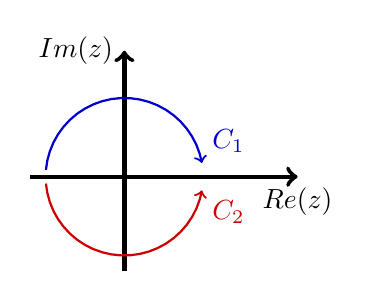
\begin{tikzpicture}
    \draw[ultra thick,->] (-1.2,0) -- (2.2, 0) node[below] {$Re(z)$};
    \draw[ultra thick,->] (0,-1.2) -- (0,1.6) node[left] {$Im(z)$};
    \draw[thick,blue!80!black,domain = 175:10,variable=\t,->] plot ({cos(\t)},{ sin(\t)}) node[above right] {$C_1$}; 
    \draw[thick,red!80!black,domain = 185:350,variable=\t,->] plot ({cos(\t)},{ sin(\t)}) node[below right] {$C_2$}; 
    \end{tikzpicture}
    \end{center}
    \end{minipage}
    \item[($\ast$)] \textit{Bonus:} Repeat parts (a) and (b) for the function $h(z) = z^{1/2}$.\\
    \textit{Note:} You may need to make some `executive decisions' to make sure your problem is well-posed.
\end{enumerate}


\newpage

% Project for Integration Workshop. Dept. Mathematics. UArizona
% Write a first-order ODE solver for a system of ODEs

\section{First-order ODE Integrators}
Consider the differential equation
\begin{equation}
\label{eq:ode_system}
\begin{cases} \dot{x}(t) = -y, & \quad x(0) = 1\\ \dot{y}(t) = \phantom{-}x, & \quad y(0) = 0 \end{cases}
\end{equation}
% which we can also write in matrix notation as
% \begin{equation}
% \label{eq:ode_matrix}
% \dot{\bm{x}}(t) = \begin{bmatrix*}[r] 0 & -1 \\ 1 & 0 \end{bmatrix*} \bm{x}, \quad \bm{x}(0) = \begin{pmatrix} 1\\0 \end{pmatrix}
% \end{equation}
Use pencil-and-paper to solve the ODE. Make a quiver plot. Sketch solutions.\\

In this project, you will build a numerical solver for differential equations like this one. You will test your solver on this ODE, and then use it to solve a more interesting ODE.
For this problem, discretize the time interval $0 \leq t \leq T$ into $n+1$ points. That is, set $\Delta t = T/n$ and $t_k = k \, \Delta t$, so $ t = \{t_0, t_1, \dots, t_n\}$. \\
\textit{Forward Differences:}
\begin{enumerate}[(a)]
    \item Use what's called a \textit{first-order forward difference} approximation to the derivatives $\dot{x}$ and $\dot{y}$ at each $t$ as follows:
    \begin{equation} 
    \label{eq:forward_difference}
    \dot{x}(t) \approx \frac{x(t + \Delta t) - x(t)}{\Delta t} \qquad \text{and} \qquad \dot{y}(t) \approx \frac{y(t + \Delta t) - y(t)}{\Delta t}.
    \end{equation}
     Substitute equation (\ref{eq:forward_difference}) into equation (\ref{eq:ode_system}) and show that we can approximate the differential equation by the discrete time-stepping process:
    \begin{equation}
    \label{eq:forward_euler}
    \begin{cases} x_{k+1} = x_k - (\Delta t) y_k, & \quad x_0 = 1\\  y_{k+1} = y_k + (\Delta t) x_k, & \quad y_0 = 0\\  \end{cases}
    \end{equation}
    \item Implement equation \ref{eq:forward_euler} for $0 \leq t \leq 1$ and plot the trajectory given by the solution.
    \item Is your approximation qualitatively correct? Will it remain qualitatively correct on $0 \leq t \leq T$ as $T$ gets very large? Explain.\\
    \textit{Hint:} It may be useful to rewrite the system of difference equations in matrix form,
    \begin{equation*}
    \bm{x}_{k+1} 
    % = \bm{x}_n + (\Delta t) \begin{bmatrix*}[r] 0 & -1 \\ 1 & 0 \end{bmatrix*} \bm{x}_n 
    = \begin{bmatrix} 1 & -\Delta t \\  \Delta t & 1\end{bmatrix} \bm{x}_k, \quad \bm{x}_0 = \begin{pmatrix} 1\\0 \end{pmatrix}
    \end{equation*}
    and to analyze the eigenvalues of the matrix.
\end{enumerate}
\textit{Backward Differences:}
\begin{enumerate}[(a),resume]
    \item We could have solved this problem by a different approach. We could also have used what's called a \textit{first-order backward difference}:
    \begin{equation} 
    \label{eq:backward_difference}
    \dot{x}(t) \approx \frac{x(t) - x(t - \Delta t)}{\Delta t} \qquad \text{and} \qquad \dot{y}(t) \approx \frac{y(t) - y(t  \Delta t)}{\Delta t}.
    \end{equation}
    Show that the backward difference gives the approximation
    \begin{equation}
    \label{eq:backward_euler}
     \begin{cases} x_{k} = x_{k-1} - (\Delta t) y_k, & \quad x_0 = 1\\  y_{k} = y_{k-1} + (\Delta t) x_k, & \quad y_0 = 0\\  \end{cases}
    \end{equation}
    which can be rewritten as
   \begin{equation*} 
    \bm{x}_{k} 
    % = \bm{x}_n + (\Delta t) \begin{bmatrix*}[r] 0 & -1 \\ 1 & 0 \end{bmatrix*} \bm{x}_n 
    = \left(\begin{bmatrix} 1 & \Delta t \\  -\Delta t & 1\end{bmatrix}\right)^{-1} \bm{x}_{k-1}, \quad \bm{x}_0 = \begin{pmatrix} 1\\0 \end{pmatrix}
    \end{equation*}
    \item Implement equation (\ref{eq:backward_euler}) for $0 \leq t \leq 1$ and plot the trajectory given by the solution. 
    \item Is your approximation qualitatively correct? Will it remain qualitatively correct on $0 \leq t \leq T$ as $T$ gets very large? Explain.
\end{enumerate}
\textit{Bonus:}
\begin{enumerate}[(a),resume]
    \item (The really fun stuff) Use your ODE solver to solve $\dot{x} = -y$, $\dot{y} = \sin x$. 
\end{enumerate}
\newpage



\newpage

\section{Random Walk on a Grid} 
A `particle' takes a random walk on a $4 \times 8$ grid. At each step of the walk, the particle may move up, down, left, or right with equal probability. The particle continues this process until it exits the grid. If the particle exits the top of the grid, the particle scores 1 point for the walk. If the particle exits the left, bottom or right sides of the grid, the particle scores 0 points for the walk. 
Compute the expected score of the particle as a function of the starting coordinates.\\

\noindent \textit{Hint:} For each starting point, you may estimate the expected score of the particle by simulating many, many random paths and taking their average score.\\
\begin{center}
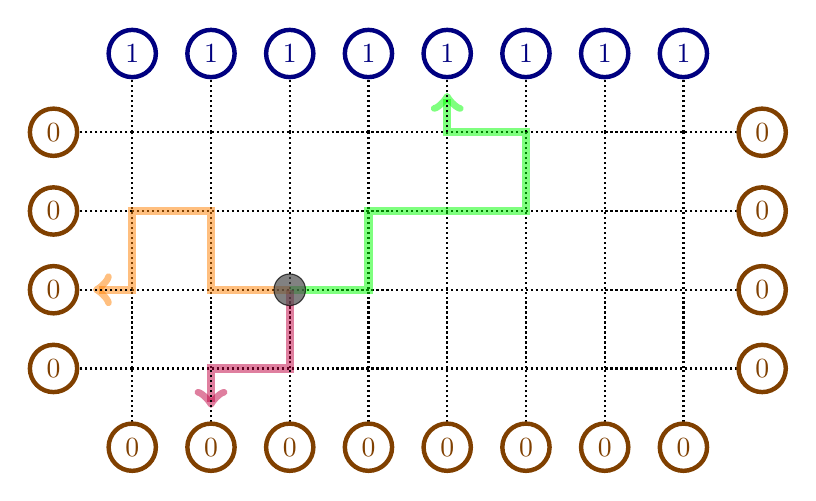
\begin{tikzpicture}
    \pgfmathsetmacro{\N}{8}
    \pgfmathsetmacro{\M}{4}
    \draw[thick, densely dotted] (1,1) grid (\N,\M);
    \draw[line width = 3,color = green, opacity = .5,->] (3,2) -- (4,2) --(4,3) --(5,3) -- (6,3) --(6,4) --(5,4) -- (5,4.5);
    \draw[line width = 3,color = purple, opacity = .5,->] (3,2) -- (3,1) --(2,1) --(2,0.5);
    \draw[line width = 3,color = orange, opacity = .5,->] (3,2) -- (2,2) --(2,3) --(1,3) -- (1,2)--(0.5,2);
    % Right
    \foreach \j in {1,...,\M}
    {
    \draw[thick, densely dotted] (\N+1,\j) -- (\N,\j);
    \draw[ultra thick,color=orange!50!black,fill = white] (\N+1,\j) node {0} circle (.3);
    }
    % Top
    \foreach \i in {1,...,\N}
    {
        \draw[thick, densely dotted] (\i,\M) -- (\i,\M+1);
        \draw[ultra thick,color=blue!50!black,fill = white] (\i,\M+1) node {1} circle (.3);
    }
    % Left
    \foreach \j in {1,...,\M}
    {
        \draw[thick, densely dotted] (1,\j) -- (0,\j);
        \draw[ultra thick,color=orange!50!black,fill = white] (0,\j) node {0} circle (.3);
    }
    % Bottom
    \foreach \i in {1,...,\N}
    {
        \draw[thick, densely dotted] (\i,0) -- (\i,1);
        \draw[ultra thick,color=orange!50!black,fill = white] (\i,0) node {0} circle (.3);
    }
    \draw[color = black,fill=black!70!white,opacity = .7] (3,2) circle  (.2);
\end{tikzpicture}
\end{center}
The figure shows three sample paths of the random walk that all begin at the initial point (3,2). For the red path, the particle (randomly) takes the steps $(\downarrow, \leftarrow, \downarrow)$, and exits the grid at the bottom scoring zero points for the walk. The other paths are the results of the steps listed below
\begin{align*}
&\text{Steps: }  (\downarrow \ \leftarrow \ \downarrow) &&\text{(See red path)} && \text{Exit: Bottom} && \text{Score: 0}\\
&\text{Steps: }  (\leftarrow \ \uparrow \ \leftarrow \ \downarrow \ \leftarrow) &&\text{(See orange path)} && \text{Exit: Left} && \text{Score: 0}\\
&\text{Steps: }  (\rightarrow \ \uparrow \ \rightarrow \ \rightarrow \ \uparrow \ \leftarrow \ \uparrow) &&\text{(See green path)}&& \text{Exit: Top} && \text{Score: 1}
\end{align*}



\noindent\textit{Bonus:} In this project, we have computed the solution to a problem by simulating many random events. This `indirect' approach is always computationally inefficient, so it is often worth looking for a `direct' approach. For this problem, there \textit{is} a method of computing the solution directly. Can you find it?


\newpage

\section{Bias and Variance of fitting a function in 1-D}

Let $f(x) = x^2(1-x)$ where $0 \leq x \leq 1$. We wish to find the `best' linear model (or approximation) for $f$. That is, for functions in the form $g(x; \alpha, \beta) =  \alpha +  \beta x$,  we wish to find the parameters $ \alpha$ and $ \beta$ that minimize the error we would expect to incur if we used the function $g$ to model (or approximate) the function $f$. 
\begin{center}
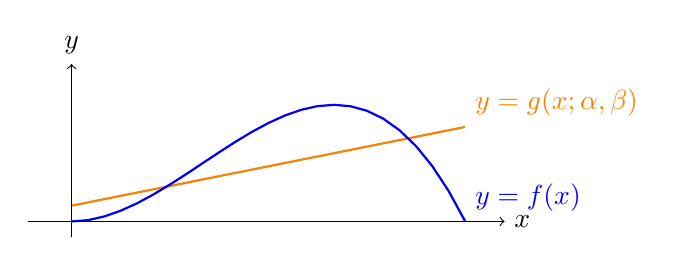
\begin{tikzpicture}[xscale=5,yscale=10]
% \draw[densely dotted] (-.2,-.2) grid (1.2,0.3);
\draw[thick,domain=0:1,variable=\x,orange] plot ({\x},{.02 + .1*\x}) node[above right] {$y = g(x; \alpha, \beta)$};
\draw[thick,domain=0:1,variable=\x,blue] plot ({\x},{\x*\x*(1-\x)}) node[above right] {$y = f(x)$};
  \draw[->] (-.11, 0) -- (1.1, 0) node[right] {$x$};
  \draw[->] (0, -.02) -- (0, .2) node[above] {$y$};
\end{tikzpicture}
\end{center}
For this problem, we will define the error as
\begin{equation*}
\text{Error}(f,g) = \int_0^1 \bigg(f(x) - g(x; \alpha, \beta)\bigg)^2 dx.
\end{equation*} 
Use pencil-and-paper (or Mathematica, WolframAlpha, etc) to find a simplified expression for the error between $f$ and $g$ as a function of the parameters $ \alpha$ and $ \beta$. Find the values of $ \alpha$ and $ \beta$ that minimize this error.

% (where the notation $y = g(x; \alpha, \beta)$ to denote a function of a single variable, namely $x$, that depends on two parameters, namely $ \alpha$ and $ \beta$).
\textit{Terminology:} The error we expect to incur when we use our best possible candidate is called the \textit{bias} of the model.


In many practical applications, we only have imperfect knowledge of $f$, and therefore it is impossible to know the parameters of the \textit{best possible} candidate $g(x, \alpha, \beta)$. Often, we must commit to a choice of sub-optimal parameters that are chosen after only a small glimpse of $f$. In this project, we will estimate how much more error we expect to incur by using an imperfect choice of parameters.


Repeat the following recipe to estimate how well a linear function parameterized by two random data points can be used to approximate $f$.\\
\texttt{Loop until you are confident you have reasonably accurate answers.}
\begin{enumerate}\setlength{\itemsep}{0pt}
    \item \texttt{Generate two random data points on $x_1, x_2 \in [0,1]$.}
    \item \texttt{Using \textbf{only} $x_1$ and $x_2$, compute a `best guess' for parameters $\alpha$ and $\beta$.}
    \item \texttt{Test the performance of your (sub-optimal) parameters by generating new data points and computing the mean square error on the new points. Record the mean square error.}
\end{enumerate}
\texttt{Analyze the expected error by taking averages and plotting histograms.}

% \textit{Terminology:} The `extra error' that we expect to typically incur by using `best guess' parameters is called the variance of the model. \\
\textit{Terminology:} When we use `best guess' parameters instead of `best possible' parameters, we can expect to incur error beyond the bias of the model. This `extra error' is called the \textit{variance} of the model.  

For this project, you will need to write the following functions:
\begin{enumerate}
    \item a function that randomly generates two values in $[0,1]$
    \item a function called \texttt{train\_g}.
    \begin{itemize}
        \item Arguments (Input): Two values $x_1$, and $x_2$.
        \item Functionality: Evaluate $y_1:=f(x_1)$ and $y_2:= f(x_2)$. Compute a `best guess' for the parameters $ \alpha$ and $ \beta$ given the points $(x_1,y_1)$ and $(x_2,y_2)$.
        \item Return (Output): $ \alpha$ and $ \beta$.
    \end{itemize}
    \item a function called \texttt{test\_g}.
    \begin{itemize}
        \item Arguments (Input): Parameters $ \alpha$ and $ \beta$.
        \item Functionality: Randomly pick $N$ points in $[0,1]$. For each point, $x_k$, evaluate $f(x_k)$ and $g(x_k;  \alpha,  \beta)$. Compute the average error from the $N$ points as defined by $$E_N = \frac{1}{N}\sum_{k = 1}^N \Big(f(x_k) - g(x_k, \alpha, \beta)\Big)^2$$
        \item Return (Output): $E_N$   
    \end{itemize}
\end{enumerate}

Someone proposes that the variance is so big that it makes the linear model unusable.  They suggest that we should approximate $f$ by a constant function  $h(x;\alpha)$. Compute the new bias, and the estimate the new total error. 

\newpage

\section{Random Triangles in High Dimensions}

For a triangle $\Delta$, we will let $\mathcal{Q}$ be a measure of the \textit{quality} of the triangle as defined by
\begin{equation}
\label{eq:triangle_score}
\mathcal{Q}(\Delta) = \frac{3\sqrt{2} A}{ \ell_1^2 + \ell_2^2 + \ell_3^2}
\end{equation}
where $A$ is the area of the triangle, and $\ell_1$, $\ell_2$ and $\ell_3$ are the lengths of the three sides.
Without performing any computations, can you determine the maximum and minimum values that $\mathcal{Q}$ can take? Can you describe what kinds of triangles are associated with high, and with low, values of $\mathcal{Q}$?

In the first part of this project, you will write a function that computes the quality of a triangle in $\mathbb{R}^2$, given the coordinates of its vertices.

\begin{enumerate}[(a)]
  \item Write a function, \texttt{tri\_lengths()}, that takes as its arguments the three vertices of a triangle and returns the lengths of the three sides of the triangle.  
  \item Write a function, \texttt{tri\_angles()}, that takes as its arguments the three vertices of a triangle and returns the angles of the triangle.
  \item Write a function, \texttt{tri\_area()}, that takes as its arguments the three vertices of a triangle and returns the area of the triangle.
  \item Write a function, \texttt{tri\_score()}, that takes as its arguments the three vertices fo a triangle and returns the quality score of the triangle as defined in equation (\ref{eq:triangle_score}). 
  \item Test your function \texttt{tri\_score()} on the four triangles below. As a check on your function, the correct values are $\mathcal{Q}({\color{red}{\Delta}}) = ....$, $\mathcal{Q}({\color{green}{\Delta}}) = ...$, $\mathcal{Q}({ \color{purple}{\Delta}}) = ...$, and $\mathcal{Q}({ \color{blue}{\Delta}}) = ...$.
\end{enumerate}

\begin{center}
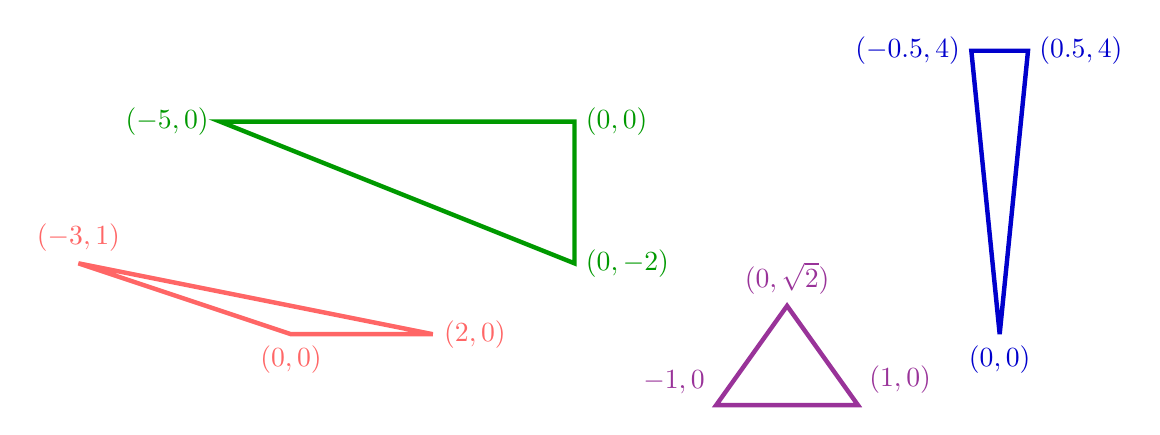
\begin{tikzpicture}[scale = 1.8]
  \draw[ultra thick,red!60!white] (0,0)node[below] {$(0,0)$} -- (-1.5,.5)node[above]{$(-3,1)$} -- (1,0)node[right]{$(2,0)$} --cycle;
  \draw[ultra thick, green!60!black] (-0.5,1.5)node[left] {$(-5,0)$} -- (2,1.5)node[right]{$(0,0)$} -- (2,.5)node[right]{$(0,-2)$} -- cycle;
  \draw[ultra thick, red!50!blue!80] (3,-.5)node[above left] {$-1,0$} -- (4,-.5)node[above right] {$(1,0)$} -- (3.5,.2)node[above]{$(0,\sqrt{2})$} -- cycle;
  \draw[ultra thick, blue!80!black] (5,0)node[below]{$(0,0)$} -- (4.8,2)node[left]{$(-0.5,4)$} -- (5.2,2)node[right]{$(0.5,4)$} -- cycle;
\end{tikzpicture}
\end{center}

Many applied mathematicians regularly work with data sets where each data point is associated with many different features (e.g. each medical patient is associated with their own temperature, heart rate, blood pressure, etc). 
Sometimes the intuition we have derived from the physical, three-dimensional world carries over to higher dimensional space. More often, we fail to grasp all the weird ways that the higher dimensional space is `bigger'. 

In the second part of this project, you will compare the expected quality $\mathcal{Q}$ of random triangles in $\mathbb{R}^2$ with that of random triangles in $\mathbb{R}^{10}$.
\begin{enumerate}[(a)]
  \item 
  \begin{enumerate}[i.]
    \item Use a random number generator to create a random point, \(\bm{x} = (x_1,x_2)\), that is normally distributed in $\mathbb{R}^2$. The functions \texttt{randn()} (Matlab), \texttt{np.random.randn()} (Python), or \texttt{randn()} (Julia) may be useful.
    \item Repeat part i. until you have three points, $\bm{x} = (x_1,x_2)$, \(\bm{y} = (y_1,y_2)\), and \(\bm{z} = (z_1,z_2)\). Consider the triangle, $\Delta$, formed by the three points as its vertices. Use your function \texttt{tri\_score()} to compute $\mathcal{Q}(\Delta)$.
    \item Repeat parts i. and ii. until you have the quality scores for 1000 random triangles. Plot a histogram of your data.
  \end{enumerate}
  \item Repeat this process for triangles in $\mathbb{R}^{10}$. That is, use a multivariate normal random number generator to generate 3 points in $\mathbb{R}^{10}$, $\bm{x} = (x_1,x_2,\dots x_{10})$, $\bm{y} = (y_1,y_2,\dots,y_{10})$, $\bm{z} = (z_1,z_2, \dots, z_{10})$. Let $\Delta$ be the triangle with $\bm{x}$, $\bm{y}$, and $\bm{z}$ as its vertices, and compute $\mathcal{Q}(\Delta)$. Repeat for 1000 random triangles.
 \item Compare the histogram for triangles in $\mathbb{R}^2$ with a histogram for triangles in $\mathbb{R}^{10}$. 
\end{enumerate}
Provide a geometric explanation for why the random triangles in higher dimensions are much closer to equilateral than the random triangles in lower dimensions

\newpage

\end{document}
\section{The Fredholm Alternative \& Least squares solutions}
Sometimes we focus too much on solving the matrix equation $A \bm{x} = \bm{b}$ for situations where $A$ is a square matrix,  and we ignore situations where $A$ is not square. In many practical applications,  $A$ is an $m \times n$ matrix with $m \neq n$. In this problem, we're going to explore what we mean by \textit{solutions to the matrix equation for non-square matrices}.

\subsubsection*{The Fredholm Alternative}
The Fredholm alternative states that for the matrix equation $Ax=b$, exactly one of the following statements is true:
\begin{itemize}
    \item (Either) There exists an $x$ that solves the matrix equation $Ax=b$.
    \item (Or) There exists a $y$ that solves $A^\top y = 0$ such that $y^\top b \neq 0$.
\end{itemize}
Let $A_m$ be the $3 \times m$ matrix (below), and let $b'$ and $b''$ be the $3 \times 1$ vectors (below).
\begin{equation*}
A_m = \begin{bmatrix} 1 & 1 & 1 & \cdots & 1\\ 1 & 1 & 1 & \cdots & 1 \\ 1 & 2 & 3 &  \cdots & m \end{bmatrix}, \quad  \quad b' = \begin{bmatrix} -1 \\ -1 \\ +1 \end{bmatrix}, \quad b'' = \begin{bmatrix*}[r] -1 \\ 0 \\ +1 \end{bmatrix*}
% A_n = \begin{bmatrix} 1 & 1 & 1 \\ 1 & 1 & 2 \\ \vdots & \vdots & \vdots \\ 1 & 1 & n \end{bmatrix}, \quad  \quad b_1 = \begin{bmatrix} 0 & 0 & -1 \end{bmatrix}, \quad b_2 = \begin{bmatrix} 1 \\ -1 \\ 0 \end{bmatrix}
\end{equation*}

\begin{enumerate}[(a)]
    \item Plot the vectors that make the columns of $A_m$ for $m = 5$, and use your figure to describe the column space of $A_m$.
    \item Use pencil-and-paper to verify the Fredholm Alternative for $b'$ and for $b''$.
    \item Plot the vectors $b'$ and $b''$ on the same figure from part (a), and use your figure to provide an intuitive explanation for the Fredholm Alternative.
\end{enumerate}

\subsubsection*{Pseudo-inverses \& Least Squares Solutions}
When there is no solution to the matrix equation $Ax = b$, we may have to make and `executive decision' and work with the `next best thing'. Your co-worker suggests the following matrix-algebra to find the `next best thing'.
\begin{equation*}
Ax = b \quad \Rightarrow \quad A^\top A x = A^\top b \quad \Rightarrow \quad x = (A^\top A)^{-1} A^\top b
\end{equation*}
\begin{enumerate}[(a), resume]
    \item What are the dimensions of the matrix $(A^\top A)$? What are requirements on $A$ for the matrix $(A^\top A)$ to be invertable?
    \item For $m = 2$, find the matrix $A^\dagger:=(A_m^\top A_m) A_m^\top$ and compute the vectors $x': = A^\dagger b'$ and $x'':=A^\dagger b''$.
    \item Does $Ax' = b'$? What about $Ax'' = b''$? Can you describe what we mean when we say that $A^\dagger$ gives the `next best thing'?
    \item (Bonus) Use some calculus to verify your answer in part (f).
\end{enumerate}


\newpage

\section{Lagrange interpolating polynomials for function approximation}
Let $\{(x_k,y_k) , k = 1, \dots, N\}$ be $N$ points in $\mathbb{R}^2$ that satisfy $x_k \neq x_j$ whenever $k \neq j$, the \textit{Lagrange Interpolating polynomial} is defined as
\begin{equation}
L(x) = \sum_{k = 1}^N \left(\prod_{j \neq k}\frac{x-x_j}{x_k-x_j} \right) y_k.
\end{equation}
We wish to determine how well a Lagrange Interpolating polynomial can approximate the functions 
\begin{equation}
f(x) = (x-.9)(x-.4)(x+.1)(x+.7)(x+.8)
\end{equation}
and 
\begin{equation}
g(x) = \frac{1}{1+10x^2} \quad \quad \text{for } -1 \leq x \leq 1
\end{equation}
\begin{enumerate}[(a)]
    \item The Lagrange interpolating polynomial is linear combination of $N$ terms in the form
    \begin{equation}
    T_k(x): =\left( \prod_{j \neq k}\frac{x-x_j}{x_k-x_j}  \right) 
    \end{equation}
    Let $x_1= -1$, $x_2 = 0$, and $x_3 = 1$. Plot the functions $T_k(x)$ for $k = 1,\dots,3$, and describe what you see.
    \item 
    \begin{enumerate}[i.]
      \item Sample $f(x)$ at the points $x_1 = -1$, $x_2 = 0$, and $x_3= 1$. Compute and plot the Lagrange Interpolating polynomial given by these 3 equi-spaced points.
      \item Repeat part (b)(i) with 5 equi-spaced points, and again with 9 equi-spaced points. Plot your results and describe whether your approximation improves with more points. 
    \end{enumerate}
    \item Repeat part (b) for the function $g(x)$.
    \item There is a well-known rule of thumb for improving numerical approximations: Sample your function with a higher density of sample points in regions where the error is biggest. Does this rule of thumb seem to work with the functions $f$ and $g$?
\end{enumerate}


\newpage

\section{Contour Integration of a Complex-valued Function}
\textit{(This problem is probably out of reach for students who not yet taken a course in complex analysis. No worries, we will cover this topic during the first few weeks of Math 583A.)}\\

\noindent Consider the functions $f:\mathbb{C} \to \mathbb{C}$ and $g:\mathbb{C} \to \mathbb{C}$ defined as
\begin{equation*}
f(z) = z^2 \quad \quad \text{and} \quad \quad g(z) = z^{-1}
\end{equation*}
\begin{enumerate}[(a)]
    \item Plotting:
    \begin{enumerate}[i.] 
        \item Make a surface plot showing $Re(f(z))$ and a surface plot showing $Im(f(z))$
        \item Make a surface plot showing $Re(g(z))$ and a surface plot showing $Im(g(z))$
    \end{enumerate}
    \textit{Since $g$ is undefined at $z = 0$ and since it is radially symmetric, the surface plots for $g$ can look scary when done in cartesian co-ordinates. You may try switching to polar coordinates to make prettier plots}
    \item     We can approximate the line integral (or contour integral) of a function along a curve by discretizing the curve into $N+1$ points $z(s) \to \{z_0, z_1, z_2, \dots, z_N\}$ and then computing the sum:
    \begin{equation*}
    \int_{z_o}^{z_t} f(z) dz \approx \sum_{k = 1}^{N} f(z_k) \ (z_{k} - z_{k-1})
    \end{equation*}
    \begin{minipage}{.7\textwidth}
    Define the two curves:
    \begin{align*}
    C_1:&  \quad \text{The upper half circle of radius 1 centered at $z=0$.}\\
    C_2:&  \quad \text{The lower half circle of radius 1 centered at $z=0$.}
    \end{align*}
    Approximate the line integrals of $f$ and of $g$ along the curves $C_1$ and $C_2$.
    \end{minipage}
    \begin{minipage}{.29\textwidth}
    \begin{center}
    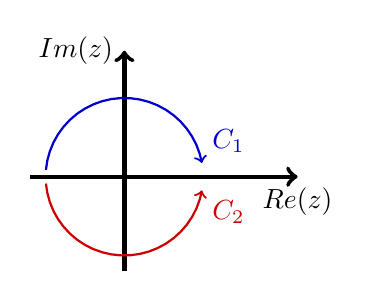
\begin{tikzpicture}
    \draw[ultra thick,->] (-1.2,0) -- (2.2, 0) node[below] {$Re(z)$};
    \draw[ultra thick,->] (0,-1.2) -- (0,1.6) node[left] {$Im(z)$};
    \draw[thick,blue!80!black,domain = 175:10,variable=\t,->] plot ({cos(\t)},{ sin(\t)}) node[above right] {$C_1$}; 
    \draw[thick,red!80!black,domain = 185:350,variable=\t,->] plot ({cos(\t)},{ sin(\t)}) node[below right] {$C_2$}; 
    \end{tikzpicture}
    \end{center}
    \end{minipage}
    \item (Bonus) Repeat (1) and (2) for the function $h(z) = z^{1/2}$.\\
    \textit{Note:} You may need to make some `executive decisions' to make sure your problem is well-posed.
\end{enumerate}

\newpage
\section{Forward-Euler Integrator}
Consider the differential equation
\begin{equation}
\label{eq:ode_system}
\begin{cases} \dot{x}(t) = -y, & \quad x(0) = 1\\ \dot{y}(t) = \phantom{-}x, & \quad y(0) = 0 \end{cases}
\end{equation}
% which we can also write in matrix notation as
% \begin{equation}
% \label{eq:ode_matrix}
% \dot{\bm{x}}(t) = \begin{bmatrix*}[r] 0 & -1 \\ 1 & 0 \end{bmatrix*} \bm{x}, \quad \bm{x}(0) = \begin{pmatrix} 1\\0 \end{pmatrix}
% \end{equation}
(Warm-up) Use pencil-and-paper to solve the ODE. Make a quiver plot. Sketch solutions.\\
(Project) We wish to build a numerical solver for differential equations like this one. We will test our solver on this ODE, and then use it to solve a more interesting ODE.

For this problem, we will discretize the time interval $0 \leq t \leq T$ into $n+1$ points, $ t = \{t_0, t_1, \dots, t_n\}$ with $t_k = k (\Delta t)$ so $t_0=0$ and $t_n = T$. 
\begin{enumerate}[(a)]
    \item For suitably small $\Delta t$ (say $\Delta t = 0.1$), we can make what's called a \textit{first-order forward difference} approximation of the derivatives $\dot{x}$ and $\dot{y}$ at each $t$ as follows:
    \begin{equation} 
    \label{eq:forward_difference}
    \dot{x}(t) \approx \frac{x(t + \Delta t) - x(t)}{\Delta t} \qquad \text{and} \qquad \dot{y}(t) \approx \frac{y(t + \Delta t) - y(t)}{\Delta t}.
    \end{equation}
     Substitute equation (\ref{eq:forward_difference}) into equation (\ref{eq:ode_system}) to show that we can approximate the differential equation by the discrete time-stepping process:
    \begin{equation}
    \label{eq:forward_euler}
    \begin{cases} x_{k+1} = x_k - (\Delta t) y_k, & \quad x_0 = 1\\  y_{k+1} = y_k + (\Delta t) x_k, & \quad y_0 = 0\\  \end{cases}
    \end{equation}
    Implement equation \ref{eq:forward_euler} for $0 \leq t \leq 1$ and plot the trajectory given by the solution. Is this approximation qualitatively correct? Will it remain qualitatively correct on $0 \leq t \leq T$ as $T$ gets very large? Explain.\\
    \textit{Hint:} It may be useful to rewrite the system of difference equations in matrix form,
    \begin{equation*}
    \bm{x}_{k+1} 
    % = \bm{x}_n + (\Delta t) \begin{bmatrix*}[r] 0 & -1 \\ 1 & 0 \end{bmatrix*} \bm{x}_n 
    = \begin{bmatrix} 1 & -\Delta t \\  \Delta t & 1\end{bmatrix} \bm{x}_k, \quad \bm{x}_0 = \begin{pmatrix} 1\\0 \end{pmatrix}
    \end{equation*}
    and to analyze the eigenvalues of the matrix.
    \item We could have solved this problem by a different approach. We could also have used what's called a \textit{first-order backward difference}:
    \begin{equation} 
    \label{eq:backward_difference}
    \dot{x}(t) \approx \frac{x(t) - x(t - \Delta t)}{\Delta t} \qquad \text{and} \qquad \dot{y}(t) \approx \frac{y(t) - y(t  \Delta t)}{\Delta t}.
    \end{equation}
    Show that the backward difference gives the approximation
    \begin{equation}
    \label{eq:backward_euler}
     \begin{cases} x_{k} = x_{k-1} - (\Delta t) y_k, & \quad x_0 = 1\\  y_{k} = y_{k-1} + (\Delta t) x_k, & \quad y_0 = 0\\  \end{cases}
    \end{equation}
    which can be rewritten as
   \begin{equation*} 
    \bm{x}_{k} 
    % = \bm{x}_n + (\Delta t) \begin{bmatrix*}[r] 0 & -1 \\ 1 & 0 \end{bmatrix*} \bm{x}_n 
    = \left(\begin{bmatrix} 1 & \Delta t \\  -\Delta t & 1\end{bmatrix}\right)^{-1} \bm{x}_{k-1}, \quad \bm{x}_0 = \begin{pmatrix} 1\\0 \end{pmatrix}
    \end{equation*}
     Implement equation (\ref{eq:backward_euler}) for $0 \leq t \leq 1$ and plot the trajectory given by the solution. Is this approximation qualitatively correct? Will it remain qualitatively correct on $0 \leq t \leq T$ as $T$ gets very large? Explain.
    \item (The really fun stuff) Perhaps solve $\dot{x} = -y$, $\dot{y} = \sin x$.  Maybe this is too hard.
\end{enumerate}
\newpage

\section{Use a random walk to solve Laplace's equation on a grid } 
A `particle' takes a random walk on a $4 \times 8$ grid. At each step of the walk, the particle may move up, down, left, or right with equal probability. The particle continues this process until it exits the grid. If the particle exits the top of the grid, the particle scores 1 point for the walk. If the particle exits the left, bottom or right sides of the grid, the particle scores 0 points for the walk. 


\begin{center}
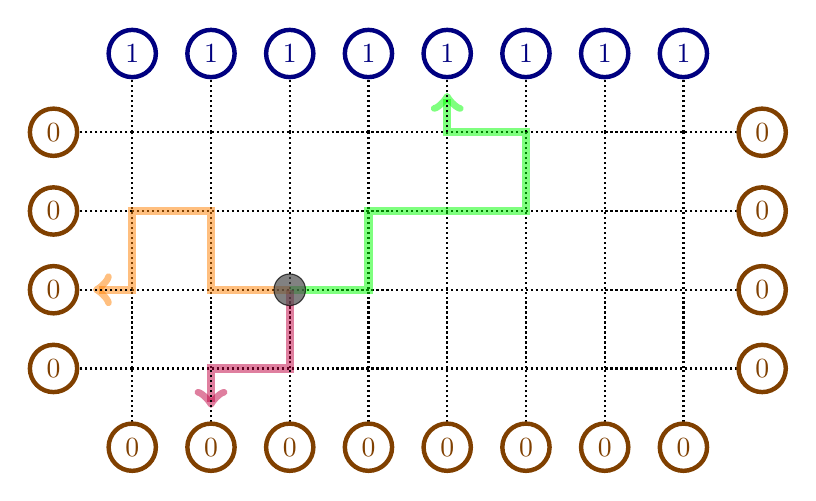
\begin{tikzpicture}
    \pgfmathsetmacro{\N}{8}
    \pgfmathsetmacro{\M}{4}
    \draw[thick, densely dotted] (1,1) grid (\N,\M);
    \draw[line width = 3,color = green, opacity = .5,->] (3,2) -- (4,2) --(4,3) --(5,3) -- (6,3) --(6,4) --(5,4) -- (5,4.5);
    \draw[line width = 3,color = purple, opacity = .5,->] (3,2) -- (3,1) --(2,1) --(2,0.5);
    \draw[line width = 3,color = orange, opacity = .5,->] (3,2) -- (2,2) --(2,3) --(1,3) -- (1,2)--(0.5,2);
    % Right
    \foreach \j in {1,...,\M}
    {
    \draw[thick, densely dotted] (\N+1,\j) -- (\N,\j);
    \draw[ultra thick,color=orange!50!black,fill = white] (\N+1,\j) node {0} circle (.3);
    }
    % Top
    \foreach \i in {1,...,\N}
    {
        \draw[thick, densely dotted] (\i,\M) -- (\i,\M+1);
        \draw[ultra thick,color=blue!50!black,fill = white] (\i,\M+1) node {1} circle (.3);
    }
    % Left
    \foreach \j in {1,...,\M}
    {
        \draw[thick, densely dotted] (1,\j) -- (0,\j);
        \draw[ultra thick,color=orange!50!black,fill = white] (0,\j) node {0} circle (.3);
    }
    % Bottom
    \foreach \i in {1,...,\N}
    {
        \draw[thick, densely dotted] (\i,0) -- (\i,1);
        \draw[ultra thick,color=orange!50!black,fill = white] (\i,0) node {0} circle (.3);
    }
    \draw[color = black,fill=black!70!white,opacity = .7] (3,2) circle  (.2);
\end{tikzpicture}
\end{center}
The figure shows three sample paths of the random walk that all begin at the initial point (3,2). For the red path, the particle (randomly) takes the steps $(\downarrow, \leftarrow, \downarrow)$, and exits the grid at the bottom scoring zero points for the walk. The other paths are the results of the steps listed below
\begin{align*}
&\text{Steps: }  (\downarrow \ \leftarrow \ \downarrow) &&\text{(See red path)} && \text{Exit: Bottom} && \text{Score: 0}\\
&\text{Steps: }  (\leftarrow \ \uparrow \ \leftarrow \ \downarrow \ \leftarrow) &&\text{(See orange path)} && \text{Exit: Left} && \text{Score: 0}\\
&\text{Steps: }  (\rightarrow \ \uparrow \ \rightarrow \ \rightarrow \ \uparrow \ \leftarrow \ \uparrow) &&\text{(See green path)}&& \text{Exit: Top} && \text{Score: 1}
\end{align*}

Compute the expected score of the particle as a function of the starting coordinates.\\

\textit{Hint:} For each starting point, you may estimate the expected score of the particle by simulating many, many random paths and taking their average score.\\

\noindent\textit{Bonus:} In this project, we have computed the solution to a problem by simulating many random events. This `indirect' approach is always computationally inefficient, so it is often worth looking for a `direct' approach. For this problem, there \textit{is} a method of computing the solution directly. Can you find it?

\newpage

\section{Bias and Variance of fitting a function in 1-D}

Let $f(x) = x^2(1-x)$ where $0 \leq x \leq 1$. We wish to find the `best' linear model (or approximation) for $f$. That is, for functions in the form $g(x; \alpha, \beta) =  \alpha +  \beta x$,  we wish to find the parameters $ \alpha$ and $ \beta$ that minimize the error we would expect to incur if we used the function $g$ to model (or approximate) the function $f$. 
\begin{center}
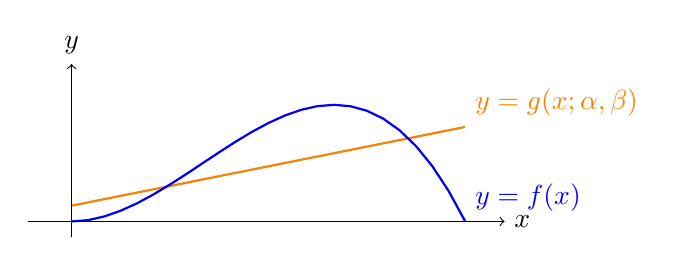
\begin{tikzpicture}[xscale=5,yscale=10]
% \draw[densely dotted] (-.2,-.2) grid (1.2,0.3);
\draw[thick,domain=0:1,variable=\x,orange] plot ({\x},{.02 + .1*\x}) node[above right] {$y = g(x; \alpha, \beta)$};
\draw[thick,domain=0:1,variable=\x,blue] plot ({\x},{\x*\x*(1-\x)}) node[above right] {$y = f(x)$};
  \draw[->] (-.11, 0) -- (1.1, 0) node[right] {$x$};
  \draw[->] (0, -.02) -- (0, .2) node[above] {$y$};
\end{tikzpicture}
\end{center}
For this problem, we will define the error as
\begin{equation*}
\text{Error}(f,g) = \int_0^1 \bigg(f(x) - g(x; \alpha, \beta)\bigg)^2 dx.
\end{equation*} 
Use pencil-and-paper (or Mathematica, WolframAlpha, etc) to find a simplified expression for the error between $f$ and $g$ as a function of the parameters $ \alpha$ and $ \beta$. Find the values of $ \alpha$ and $ \beta$ that minimize this error.

% (where the notation $y = g(x; \alpha, \beta)$ to denote a function of a single variable, namely $x$, that depends on two parameters, namely $ \alpha$ and $ \beta$).
\textit{Terminology:} The error we expect to incur when we use our best possible candidate is called the \textit{bias} of the model.


In many practical applications, we only have imperfect knowledge of $f$, and therefore it is impossible to know the parameters of the \textit{best possible} candidate $g(x, \alpha, \beta)$. Often, we must commit to a choice of sub-optimal parameters that are chosen after only a small glimpse of $f$. In this project, we will estimate how much more error we expect to incur by using an imperfect choice of parameters.


Repeat the following recipe to estimate how well a linear function parameterized by two random data points can be used to approximate $f$.\\
\texttt{Loop until you are confident you have reasonably accurate answers.}
\begin{enumerate}\setlength{\itemsep}{0pt}
    \item \texttt{Generate two random data points on $x_1, x_2 \in [0,1]$.}
    \item \texttt{Using \textbf{only} $x_1$ and $x_2$, compute a `best guess' for parameters $\alpha$ and $\beta$.}
    \item \texttt{Test the performance of your (sub-optimal) parameters by generating new data points and computing the mean square error on the new points. Record the mean square error.}
\end{enumerate}
\texttt{Analyze the expected error by taking averages and plotting histograms.}

% \textit{Terminology:} The `extra error' that we expect to typically incur by using `best guess' parameters is called the variance of the model. \\
\textit{Terminology:} When we use `best guess' parameters instead of `best possible' parameters, we can expect to incur error beyond the bias of the model. This `extra error' is called the \textit{variance} of the model.  

For this project, you will need to write the following functions:
\begin{enumerate}
    \item a function that randomly generates two values in $[0,1]$
    \item a function called \texttt{train\_g}.
    \begin{itemize}
        \item Arguments (Input): Two values $x_1$, and $x_2$.
        \item Functionality: Evaluate $y_1:=f(x_1)$ and $y_2:= f(x_2)$. Compute a `best guess' for the parameters $ \alpha$ and $ \beta$ given the points $(x_1,y_1)$ and $(x_2,y_2)$.
        \item Return (Output): $ \alpha$ and $ \beta$.
    \end{itemize}
    \item a function called \texttt{test\_g}.
    \begin{itemize}
        \item Arguments (Input): Parameters $ \alpha$ and $ \beta$.
        \item Functionality: Randomly pick $N$ points in $[0,1]$. For each point, $x_k$, evaluate $f(x_k)$ and $g(x_k;  \alpha,  \beta)$. Compute the average error from the $N$ points as defined by $$E_N = \frac{1}{N}\sum_{k = 1}^N \Big(f(x_k) - g(x_k, \alpha, \beta)\Big)^2$$
        \item Return (Output): $E_N$   
    \end{itemize}
\end{enumerate}

Someone proposes that the variance is so big that it makes the linear model unusable.  They suggest that we should approximate $f$ by a constant function  $h(x;\alpha)$. Compute the new bias, and the estimate the new total error. 

\newpage


\section{Nearest neighbors can be very far away. Curse of dimensionality}

\textit{In Progress.}

\end{document}
